\documentclass[../main]{subfiles}
 
\begin{document}

\chapter{Ergodic theory and dynamics}

\section{A categorical zoo}
The starting point of the field of dynamical systems is a space \(X\), endowed with some structure, along with some notion of ``time evolution'', which could be a map \(X \to X\) preserving the said structure. For instance, in topological dynamics, \(X\) is usually a topological space and the time evolution is given by a continuous map, while in ergodic theory the space is endowed with the structure of a measure and the maps are measure-preserving. But it is also of equal interest to the field to look at more versatile settings, like the ones in which there are multiple maps --- or perhaps, the ones in which the maps do not send send each given state to a single next state, but to a set, or distribution, of future possibilities.

Of course, we could have a separate definition for each (and that is usually what we do). But it is also fun to see how general we can make a reasonable definition that still conveys what most such systems are. One interesting way to do that, which nicely bundles in a single notion the totality of the examples above, is the one of a \emph{monoid object} in a category. 

Following~\cite{mossCategorytheoreticProofErgodic2023}, we can define a monoid object in a category \(\cC\) as a functor \(M \to \cC\), where \(M\) is \emph{monoid}, that is, a category with a single object. An usual monoid is just a group without the inverse operation, namely, a set \(M\) endowed with a special identity element \(1_M\) and a multiplication \((a,b) \in X \times X \mapsto a \cdot b \in X\) satisfying
 
\begin{enumerate}[i.]
\item \(1_M \cdot a = a = a \cdot 1_M\) for all \(a \in M\);
\item \((a \cdot b) \cdot c = a \cdot (b \cdot c)\) for all \(a, b, c \in M\).
\end{enumerate}
Given such a monoid \(M\), the category composed of a single object \(\bigstar\), set of morphisms \(\Hom{}(\bigstar, \bigstar) = M\) and composition given by the monoid multiplication will satisfy the definition of a category. Conversely, any (small) category with a single object \(\bigstar\) can be seen as a monoid, by taking the carrier set to be the set \(M = \Hom{}(\bigstar, \bigstar)\) and the product, to be the composition. Let's see how many familiar examples of dynamics fit neatly in this definition.

\subsection{Examples}

\subsubsection{One map}
The simplest example is that of a set \(X\) and a map \(f \colon X \to X\).
This fits the categorical definition by taking \(\cC = \mathbf{Set}\) and \(M = \mathbb{N}\) (the natural numbers under addition, which forms a monoid). The functor \(F \colon M \to \mathbf{Set}\) sends the single object \(\bigstar\) of \(M\) to \(X\), and each morphism \(n \in \mathbb{N} = \Hom{}(\bigstar, \bigstar)\) to the \(n\)-fold composition \(f^n = f \circ f \circ \cdots \circ f\) (with \(f^0 = \mathrm{id}_X\)). The functor axioms ensure that \(F(0) = \mathrm{id}_X\) and \(F(n + m) = F(n) \circ F(m) = f^n \circ f^m = f^{n+m}\), which is precisely the monoid homomorphism property.


\subsubsection{Two maps}
To illustrate the definition, if \(f_a,f_b \colon X \to X\) are two measure-preserving maps, then the associated monoid is the one-object category for the free monoid with two generators \(\set{a,b}\), and the functor sends \(\bigstar\) to the object \(X\) and words to the compositions of \(f_a\) and \(f_b\) in the category of measure-preserving maps. For instance, the word \(abba\) is sent to the map \(f_a \circ f_b \circ f_b \circ f_a \colon X \to X\).

\subsubsection{Markov kernels}
Another example is that of Markov kernels, or Markov chains. Often, it is useful to model stochastic dynamics by having the maps send each point \(x \in X\) not to a point \(f(x) \in X\), but to a \emph{probability measure} \(f(x) \in \Meas[1]{X}\). The probability measure \(f(x)\) then encodes the distribution of expected outcomes given that we started in the state \(x\).

How we can compose iterates of \(f\) and regard it as a dynamic on \(X\)? Semantically, we want the iterates to encode the distribution of expected outcomes after \(n\) steps given that the system started at the point \(x\). To work it out, we can start with the case where \(X\) is finite, so any \(f(x)\in \Meas[1]{X}\) is completely determined by some transition probabilities \(\Prob(f(x) = y) \coloneqq f(x)(\set{y})\). Then, supposing that the probability of first making the transition \(x \mapsto y\) and then \(y \mapsto z\) is \(\Prob(f(x) = y)\cdot \Prob(f(y) = z)\), we should have
\[\displaystyle\Prob(f^2(x) = z) = \sum_{y \in X} \Prob(f(x) = y)\cdot \Prob(f(y) = z).\]
If we rewrite the above with a measure-theoretic language, we see that we ought to define
\begin{equation*}
  f^2(x)(E) = \int_X f(y)(E) \;d (f(x))\set{y}.
\end{equation*}
More generally, given \(f \colon X \to \Meas[1]{Y}\),  \(g \colon Y \to \Meas[1]{Z}\), we can define a kernel composition by
\begin{equation*}
  (g \circ f)(x)(E) = \int_X g(y)(E)\;d(f(x))\set{y}
\end{equation*}
so that \(g \circ f \colon X \to \Meas[1]{Z}\).

A map with type \(X \to \Meas[1]{Y}\) is called a \emph{Markov kernel} between the measurable spaces \(X\) and \(Y\). The category whose objects are measurable spaces and morphisms are Markov kernels, with compositions given by the rule above, will be called \(\Stoch\). We remark that the identity morphisms in this category are the Dirac masses \(\delta(x) = \delta_x \in \Meas[1]{X}\).

An interesting aspect of this category is that deterministic measurable maps still live inside it --- given \(g \colon X \to Y\) a measurable function, \(f_g(x) = \delta_y\) is a Markov kernel. That is to say, this correspondence defines a (faithful) functor from the category \(\MeasC\) of measurable functions to \(\Stoch\). This means that dynamics in \(\Stoch\) can be seen a generalization of deterministic measurable systems, where we now also allow the maps to be stochastic.

Another observation is that a probability measure \(\mu\) in a measurable space \(X\) can be represented in this category by a Markov kernel \(m \colon \set{\star} \to \Meas[1]{X}\), where \(\set{\star}\) is a measurable space with one element. Namely, we set \(m(\star) = \mu\).

% \subsubsection{Iterated function systems}\label{def:hausdorff-metric}

% Iterated functions systems are a way of constructing self-similar sets, better known as fractals. For that, we start with a complete metric space \(X\) and a finite set of contraction mappings \(\set{f_1,\dots,f_n} \subseteq X \to X\), where each \(f_i \colon X \to X\) is a contraction. The idea is to consider all the possibilities where a point \(x \in X\) could land: the union \(\bigcup_{1 \le i \le n}\set{f_i(x)}\) of all images. It is similar, in spirit, to the example of Markov Kernels above, but we consider the possibilities as a \emph{closed set}, instead of a measure.

% How would the composition work, in this case? In other words, what category are we thinking about when we consider iterates of the function system? To answer that, define the \emph{Hutchinson operator} \(F\): let \(A \subseteq X\) be a compact set, and let
% \begin{equation*}
%   F(A) = \bigcup_{1 \le i \le n} \set{f_i(A)}.
% \end{equation*}
% This set is a finite union of compact sets, so \(F(A)\) is compact. This defines a function \(F \colon \mathcal{K}(X) \to \mathcal{K}(X)\) on the set \(\mathcal{K}(X) \subseteq 2^{\cms}\) of nonempty compact subsets of \(X\). In fact, we shall endow \(\mathcal{K}(X)\) with the metric space structure given by
% \begin{equation*}
%   d_H(A,B) = \max \set[par = \big]{  \sup_{a \in A} d(a, B), \sup_{b \in B} d(A, b)},
% \end{equation*}
% which is called the Hausdorff metric.

% % \begin{lemma}
% %   Let \(U \subseteq X\) be open. Then, the set \(\set{K \in \mathcal{K}(X) \where K \subseteq U}\) is an open subset of \(\mathcal{K}(X)\).
% % \end{lemma}

% We can show \(F\) is also a contraction in this metric: we have, for \(A\) and \(B\) nonempty compact sets, 
% \begin{align*}
%   \sup_{a \in F(A)}d(a, F(B))
%   &= \sup\set[par = \bigg]{d(a, F(B)) \where a \in \bigcup_{1 \le i \le n} f_i(A)}\\
%   &\le \max_{1 \le i \le n} \sup\set{d(f_i(a), F(B)) \where a \in A}\\
%   &\le \max_{1 \le i \le n} \sup\set{d(f_i(a), f_i(B)) \where a \in A}\\
%   &\le \lambda \sup\set{d(a, B) \where a \in A} \le \lambda d_H(A,B),
% \end{align*}
% where \(\lambda\) is the largest Lipschitz constant of the \(f_i\). Exchanging the roles of \(A\) and \(B\), we get \(d_H(F(A), F(B)) \le \lambda d_H(A,B)\), so \(F\) is a contraction with the same constant \(\lambda\).

% \todo{remove after complete}

\subsection{Invariant states and observables}

Two important concepts in the study of dynamical systems are the notions of invariant states and invariant observables. In~\cite{mossCategorytheoreticProofErgodic2023}, a systematic treatment of those objects is suggested using the categorical language which we have been developing here.

A \emph{cone} over a functor \(F \colon \cD \to \cC\) is defined as an object \(C \in \cC\) and a natural transformation \(T \colon \Delta_C \Rightarrow F\), where \(\Delta_C \colon \cD \to \cC\) is the constant functor at the identity of \(C\). In the case we are interested, \(\cD = M\) is a monoid and \(F\) is given by the dynamics. This means a cone is given as an object \(C \in \cC\) and a morphism \(c \colon C \to X\) with the property that for every \(m \in M\),
\[
  \begin{tikzcd}
    &\arrow[dl, "c", swap]C\arrow[dr, "c"]& \\[-10pt]
    X\arrow[rr,"m"] && X
  \end{tikzcd}
\]
commutes. 

A cone \((C, c)\) is \emph{universal} for \(M \to \cC\) if it is a limit of the above diagram, that is, for every other cone \((D, d)\), there is a unique arrow \(D \to C\) so that
\[
  \begin{tikzcd}
    &\arrow[ddl, "d", swap]D\arrow[d,dashed]\arrow[ddr, "d"]& \\
    &\arrow[dl]C\arrow[dr]& \\[-15pt]
    X\arrow[rr,"m"] && X
  \end{tikzcd}
\]
commutes. If a cone is to be seen as a collection of invariant states, then the universal cone is the biggest of them. An universal cone is a special case of a \emph{limit}. Since categorical limits are unique, if a universal cone exists, it is unique up to isomorphism as well.

\begin{example}
  Let \(f \colon X \to X\) be any function from a set to itself. Like in previous example, this will define a dynamical system in \(\SetC\) over the monoid \(\NNZ\), mapping \(n \in \NNZ\) to the iterate \(f^n\). If \(x \in X\) is a fixed point of \(f\), then we get a cone by defining \(C = \set{x}\) and picking the morphism \(c \colon C \to X\) to be the inclusion. Since \(x\) is a fixed point, it is clear that the associated diagram will commute. Conversely, if \((C,c)\) is a cone and \(x \in C\), then the commutativity of the triangle means \(f(c(x)) = c(x)\), and therefore \(c(x) \in X\) is a fixed point for \(f\).

  In this case, the \emph{universal} cone for \(f\), then, will correspond to the set \(\Fix{f}\) of all fixed points (which may be empty) paired with the set inclusion \(\Fix{f} \hookrightarrow X\). Any other cone will map uniquely to this set, by matching each of its points with the corresponding fixed point in \(\Fix{f}\).
\end{example}

\begin{example}
  Let \(f \colon X \to \Meas[1]{X}\) be a \emph{Markov kernel} from a measurable set to itself. Examples of cones for the associated system in \(\Stoch\) over \(\NNZ\) are \emph{stationary measures} \(m \colon \set{\star} \to \Meas[1]{X}\), that is, measures with the property that 
  \begin{equation*}
    (f \circ m)(\star) =  \int_X f(x) \;d\mu\set{x} = \mu,
  \end{equation*}
  where \(\mu = m(\star)\). In other words, the following diagram commutes in the category \(\Stoch\):
  \[
    \begin{tikzcd}
      &\arrow[dl, "m", swap]\{\star\}\arrow[dr, "m"]& \\[-10pt]
      X\arrow[rr,"f"] && X
    \end{tikzcd}
  \]
\end{example}

More generally, a kernel \(g \colon Y \to \Meas[1]{X}\) will define a cone if for every \(y \in Y\), \(g(y) \in \Meas[1]{X}\) is invariant.

% \begin{example}
%   \todo{For an iterated function system of contractions, the universal cone is the Hutchinson attractor. It is the map sending \(\star\) to the compact set \(A = \lim_{n \to \infty} H^i(x)\), which is independent of our starting point \(x\).}
% \end{example}

\section{Ergodic theory and ergodicity}
Ergodic theory is the domain of dynamical systems that study dynamics by means of invariant measures; it can be seen as the specialization of the section above to categories related to measure spaces and measure-preserving transformations. The hope is that the invariant measures are able to encode the asymptotic statistical behavior of the dynamics, even when individual points have very chaotic and unpredictable trajectories, and therefore, we should turn our attention to them. Indeed, the cornerstone theorem of the field, the Birkhoff pointwise ergodic theorem, provides a very positive answer to this hope.

\subsection{The pointwise ergodic theorem}

\begin{theorem}\label{thm:birkhoff}
  Let  \(\mu\) be an invariant probability measure and \(\phi \colon X \to \mathbb{R}\) an integrable function. Then, for \(\mu\)-almost every \(x \in X\),
  \begin{equation}\label{eq:birkhoff}
    \frac{1}{n}\sum_{i = 0}^{n - 1} \phi (f^i(x)) \to \CE[\mu]{\phi, \mathcal{I}}(x),
  \end{equation}
  where \(\mathcal{I}\) is the sub-\(\sigma\)-algebra of (strictly) invariant sets.
\end{theorem}

Below we reproduce a succinct proof of the theorem, described for example in~\cite[136]{katokIntroductionModernTheory1995}.

\begin{proof}
  Let
  \[F_n(x)= \max_{1 \le k \le n} \sum_{i = 0}^{k} \phi(f^i(x)).\]

  \begin{claim}
    \(F_{n + 1} = \phi + \max\set{0, F_n \circ f}\).
  \end{claim}
  To see this, note that \(\sum_{i = 0}^{k} \phi \circ f^i = \phi + \sum_{i = 0}^{k - 1} \phi \circ f^{i + 1}\), so
  \[F_{n + 1}
    = \phi + \max_{1 \le k \le n + 1}\sum_{i = 0}^{k - 1} \phi \circ f^{i + 1}
    = \phi + \max\set[par = \Big]{0,\max_{1 \le k \le n}\sum_{i = 0}^{k} \phi \circ f^{i + 1}}
    = \phi + \max \set{0,F_n \circ f}.
  \]

  \begin{claim}
    \(F_{n + 1} - F_n \circ f = \phi - \min\set{0, F_n \circ f}\).
  \end{claim}
  This claim follows from the previous one by rewriting
  \begin{align*}
    F_{n + 1} + \min\set{0, F_n \circ f} = \phi + \max\set{0, F_n \circ f} + \min\set{0, F_n \circ f} = \phi + F_n \circ f.
  \end{align*}
  Two very useful corollaries of the claim are that for each \(x \in X\), \(F_{n + 1}(x) - F_n(f(x))\) is a non-increasing sequence (because \(F_n(f(x))\) is non-decreasing by definition), and that if \(F_n(f(x)) \to \infty\), then the sequence will converge monotonically to \(\phi(x)\).

  Now, we define the set
  \begin{equation*}
    S = \set[par = auto]{x \in X \where F_n(x) \to + \infty}.
  \end{equation*}
  The first observation is that \(S \in \mathcal{I}\), because it is measurable and strictly invariant. Since \(\mu\) is invariant by \(f\), this implies \(\int_S F_n \circ f\;d\mu = \int_S F_n\;d\mu\). Also, the observations from the last claim show that \(F_{n + 1}(x) - F_n(f(x)) \to \phi(x)\) for \(x \in S\). Thus, by the dominated convergence theorem,
  \begin{equation}\label{eq:1}
    0 \le \int_S F_{n + 1} - F_n\;d\mu = \int_S F_{n + 1} - F_n \circ f\;d\mu \to \int_S \phi\;d\mu
  \end{equation}
  which means \(\int_S \phi\;d\mu \ge 0\).

  The second observation is that if \(x \notin S\), then \((F_n(x))_n\) is bounded above, so
  \begin{equation}\label{eq:2}
    \limsup_{n \to \infty} \frac{1}{n}\sum_{i = 0}^{n - 1} \phi(f^i(x)) \le \limsup_{n \to \infty} \frac{1}{n}F_n(x) \le 0.
  \end{equation}
  Putting the two together, we conclude that if \(\phi\) is such that \(\CE{\phi, \mathcal{I}} < 0\) almost everywhere, then by  \cref{eq:1} and the fact \(S \in \mathcal{I}\), the set \(S\) has measure zero, so  \cref{eq:2} is valid almost everywhere.

  The theorem then follows by noticing that for  any \(\varepsilon > 0\), if we replace \(\phi\) by \(\tilde{\phi} = \phi - {\CE{\phi,\mathcal{I}}} - \varepsilon\), then \(\CE{\tilde{\phi}, \mathcal{I}} < 0\), so
  \begin{equation*}
    \limsup_{n \to \infty} \frac{1}{n}\sum_{i = 0}^{n - 1} \tilde\phi(f^i(x))
    = \limsup_{n \to \infty} \frac{1}{n}\sum_{i = 0}^{n - 1} \phi(f^i(x)) - \CE{\phi,\mathcal{I}} - \varepsilon \le 0.
  \end{equation*}
  If we combine this with the analogous inequality for \(-\phi\), we get
  \begin{equation*}
    \CE{\phi,\mathcal{I}} - \varepsilon \le \liminf_{n \to \infty} \frac{1}{n}\sum_{i = 0}^{n - 1} \phi(f^i(x)) \le 
    \limsup_{n \to \infty} \frac{1}{n}\sum_{i = 0}^{n - 1} \phi(f^i(x)) \le  \CE{\phi,\mathcal{I}} + \varepsilon
  \end{equation*}
  and the result follows by letting \(\varepsilon \to 0\).
\end{proof}

The Birkhoff ergodic theorem shows that the Birkhoff averages often look much simpler than the observable itself. Indeed, \(\CE{\phi,\mathcal{I}}\) is measurable for the sub-\(\sigma\)-algebra \(\mathcal{I}\), and therefore is an invariant function: \(\CE{\phi,\mathcal{I}} \circ f = \CE{\phi,\mathcal{I}}\). If this algebra is trivial, then all the Birkhoff averages would converge to the same value. This suggests the following definition.

\begin{definition}
  We say that a measure \(\mu\) is \emph{ergodic} for \(f\) if the algebra \(\mathcal{I}\) is trivial modulo \(\mu\): for every \(A \in \mathcal{I}\), either \(\mu(A) = 0\) or \(\mu(A^{\complement}) = 0\).
\end{definition}

\section{Empirical measures}\label{sec:empirical-measures}
Let \(X\) be a compact metric space, and \(f \colon X \to X\) be a Borel measurable map. Given a point \(x \in X\), we can define a sequence of \emph{empirical measures}
\[\Emp[n](x) = \frac{1}{n} \sum_{i = 0}^{n - 1} \delta_{f^i(x)},\]
encoding the averages along the orbit of \(x\) up to a time \(n\). These measures are, indeed, uniquely defined by the property that for any observable \(\phi \colon X \to \mathbb{R}\), its integral with respect to \(\Emp[n](x)\) equals the Birkhoff average up to time \(n\): 
\begin{equation*}
  \int \phi \;d(\Emp[n](x)) = \frac{1}{n}\sum_{i = 0}^{n - 1} \phi(f^i(x)).
\end{equation*}
The direct relation to Birkhoff averages also highlights these objects as having a central role in ergodic theory. In particular, weak convergence of the empirical measures mean that asymptotically, the orbit has a well defined statistics: there is some invariant measure \(\mu\) which encode the limit of the Birkhoff averages of all continuous observables \(\phi\).

\begin{lemma}
  If \(e_n \weakto \mu\), then \(\mu\) is invariant for \(f\).
\end{lemma}

\begin{proof}
  Since \(X\) is compact and \(\mu\) is a Borel, continuous functions are dense in \(L^1(\mu)\). Therefore, it suffices to check that \(\mu(\phi) = \mu(\phi \circ f)\) for all \(\phi \in \Cs{X}\). For that, we notice that
  \begin{equation*}
    \abs{e_N(\phi) - e_N(\phi \circ f)} \le {2\max \phi}/{N},
  \end{equation*}
  and let \(N \to \infty\).
\end{proof}

Reciprocally, for each invariant measure \(\mu \in \Meas[f]{X}\), we can ask what are the points of \(X\) whose empirical measures converge to it. The set \(\mathcal{B}(\mu) \subseteq X\) of points with this property is called the \emph{basin} of the measure \(\mu\).

\begin{lemma}\label{lem:erg-iff-basin-full-meas}
  If \(\mu\) is an invariant probability for \(f\), then \(\mu(\Basin{\mu}) \in \set{0,1}\). Moreover, \(\mu(\Basin{\mu}) = 1\) if, and only if, \(\mu\) is ergodic for \(f\).
\end{lemma}

\begin{proof}
  Suppose \(\mu\) is an  ergodic for \(f\). Since \(X\) is compact, there is a sequence \(\set{\phi_i}_{i \in \NN} \subseteq \Cs{X}\) of functions that is uniformly dense in \(\Cs{X}\). By the pointwise ergodic theorem, for each \(i\) there is a full measure set \(E_i\) where \(\Emp[n](x)(\phi_i) \to \mu(\phi_i)\) for all \(x \in E_i\). Let \(E = \bigcap_{i \in \NN} E_i\), which has full measure.

  We claim that for all \(\phi \in \Cs{X}\) and \(x \in E\), we have \(\Emp[n](x)(\phi) \to \mu(\phi)\). Let \(\varepsilon > 0\) and let \(i\) be such that \(\norm{\phi - \phi_i}_{\infty} < \varepsilon\). If \(N\) is large enough that \(n \ge N\) implies \(\abs[\big]{\Emp[n](x)(\phi_i) - \mu(\phi_i)} < \varepsilon\), we have
  \[
    \abs[\big]{\Emp[n](x)(\phi) - \mu(\phi)} \le
    \abs[\big]{\Emp[n](x)(\phi_i) - \mu(\phi_i)} +
    \abs[\big]{\Emp[n](x)(\phi - \phi_i)} +
    \abs[\big]{\mu(\phi - \phi_i)} \le 3\varepsilon.
  \]
  This shows the claim. In particular, \(E \subseteq \Basin{\mu}\), and therefore \(\mu(\Basin{\mu}) = 1\).

  Now, suppose \(\mu\) is not ergodic; in this case, there exists some invariant set \(E \subseteq X\) with \(\mu(E) \in (0,1)\). For \(\varepsilon > 0\), consider a continuous function \(\phi\) with the property that \(\mu(\phi) = 1\) and \(\int_{E} \phi \;d\mu < \varepsilon\), which exists by normality and inner regularity. In one hand, for all \(x \in \Basin{\mu}\), we have \(\Emp[n](x)(\phi) \to \mu(\phi)\), so
  \[\int_{\Basin{\mu} \cap E}\Emp[n](x)(\phi)\;d\mu \to \mu({\Basin{\mu} \cap E})\mu(\phi) = \mu({\Basin{\mu} \cap E}).\]
  On the other hand, by the pointwise ergodic theorem and the fact \(\Basin{\mu}\cap E\) is invariant,
  \[\int_{\Basin{\mu} \cap E}\Emp[n](x)(\phi)\;d\mu \to
    \int_{\Basin{\mu}\cap E}\CE[\mu]{\phi, \mathcal{I}}(x)\;d\mu = 
    \int_{\Basin{\mu}\cap E}\phi(x)\;d\mu < \varepsilon.
  \]
  Therefore, \(\mu({\Basin{\mu} \cap E}) < \varepsilon\). Letting \(\varepsilon \to 0\), we have \(\mu({\Basin{\mu} \cap E}) = 0\). Exchanging \(E\) with \(E^{\complement}\), we conclude that \(\mu(\Basin{\mu}) = 0\).
  % tá muito zoado isso aqui, muito zoado....
\end{proof}

\begin{lemma}\label{prop:limiting-measures}
  Let \(X\) be a compact metric space with the Borel \(\sigma\)-algebra. For every \(x \in X\), the limit points in the weak-\(\ast\) topology of the sequence of empirical measures
  \begin{equation*}
    \Meas(x) = \set{ e_n(x) }[n \geq 0, '] = \bigcap_{i = 0}^{\infty} \set{ e_n(x) }[n \geq i,spar,closure]
  \end{equation*}
  form a compact connected subset of the invariant measures.
\end{lemma}

\begin{proof}
  The set is closed by definition, so by Banach-Alaoglu it is compact; for connectedness, suppose \(\Meas{x} = K_1 \cup K_2\) where \(K_1, K_2\) are closed and disjoint.
  Let \(\set{\phi_i}_{i \in \NN} \subseteq B_{\Cs{X}}\) be a dense subset and define
  \begin{equation*}
    d(\mu, \nu) = \sum_{i = 1}^{\infty} \frac{\lvert \mu(\phi_i) - \nu(\phi_i) \rvert}{2^{i}},
  \end{equation*}
  which is a metric inducing the weak-\(\ast\) topology on the set of probability measures (see~\ref{prop:weak-star-metrizable}). Since it is a metric, there are two open sets \(U_1 \supseteq K_1, U_2 \supseteq K_2\) with positive distance \(s > 0\) from each other. We claim \(\lim_{n \to \infty} d(\Emp[n]{x}, \Emp[n + 1]{x}) = 0\), which would contradict \(s > 0\) because the definition of \(\Meas{x}\) implies \(\Emp[n]{x} \in U_1\) and \(\Emp[n + 1]{x} \in U_2\) for infinitely many \(n\).
  Indeed,
  \begin{align*}
    d(\Emp[n](x), \Emp[n + 1](x))
    &= \sum_{i = 1}^{\infty} \frac{\abs{\frac{1}{n}\sum_{i = 0}^{n - 1}\phi_i \circ f^i(x) - \frac{1}{n + 1}\sum_{i = 0}^{n}\phi_i \circ f^i(x)}}{2^{i}}\\
    &\leq \sum_{i = 1}^{\infty} \frac{2}{n}\frac{\lVert \phi_i \rVert_{\infty}}{2^{i}} \leq \frac{2}{n} \to 0.
  \end{align*}
\end{proof}

% \section{Ergodic theorems}

% \section{Palis' conjecture}

% Jacob Palis had many dreams, and his dreams of mathematical nature were only a small part of his broader goals of developing science in the third world~\cite{pujalsPeixotosTheoremPaliss2011}.



% \todo{Describe the overall problem of generically finding finite set of limiting measures, whose basins cover almost all points of the manifold. Describe the robust counterexample to finiteness by Newhouse. Describe that the problem of historical behavior is open.}

% \begin{theorem}[\cite{newhouseDiffeomorphismsInfinitelyMany1974}]
%   Let \(M\) be a compact surface. There exists a non-empty open set \(U \subseteq \Diff^2(M)\) of non-hyperbolic diffeomorphisms. Moreover, any diffeomorphism in a dense \(G_{\delta}\)-subset of \(U\) has infinitely many sinks.
% \end{theorem}

% We note that in this context, a \emph{sink} is an attracting periodic orbit. Each sink corresponds to an ergodic measure (supported on the period orbit) whose basin is an open set, and therefore has positive volume.

% \begin{conjecture}
%   A
% \end{conjecture}

\section{Relating dynamics: extensions}

Different dynamical systems can be related to each other by the concept of \emph{factors}, or \emph{extensions}, expressing a sense in which one system is a simplification of another. In the categorical language we have been developing, an extension is a natural transformation \(F \Rightarrow G\) between two dynamical systems \(F\) and \(G\). In this situation, we then say that \(G\) is a \emph{factor} of \(F\). The single morphism \(F(\star) \to G(\star)\) specified by the natural transformation is also called the \emph{factor map}.

\begin{definition}
  Let \(F,G \colon M \to \Cat{C}\) be two dynamical systems on the category \(\Cat{C}\). An extension \(\eta \colon F \Rightarrow G\) consists of a morphism \(\eta \colon F(\star) \to G(\star)\) of \(\Cat{C}\) (the factor map), such that for all \(m \in M\), the diagram
  \begin{equation*}
    \begin{tikzcd}
      F(\star) \arrow[r, "F(m)"] \arrow[d, "\eta"] & F(\star) \arrow[d, "\eta"] \\
      G(\star) \arrow[r, "G(m)"] & G(\star)
    \end{tikzcd}
  \end{equation*}
  commutes.
\end{definition}

Now, we conclude our tour around the zoo and focus on our beloved species, measure-preserving systems.

\begin{definition} Let $(X, \mathcal{B}_X, \mu, f)$ and $(Y,\mathcal{B}_Y, \nu, g)$ be measure-preserving transformations. 
  $(Y,\mathcal{B}_Y, \nu, g)$ is a \textbf{factor} of $(X, \mathcal{B}_X, \mu, f)$ if there exists a measure-preserving map $\phi: X \to Y$ such that 
  \[
    \begin{tikzcd}
      X \arrow[r, "f"] \arrow[d, "\phi"] & X \arrow[d, "\phi"] \\
      Y \arrow[r, "g"] & Y
    \end{tikzcd}
  \]
  commutes.
\end{definition}
  

\begin{example}
  Every system admits a trivial factor:
  \[
    \begin{tikzcd}
      X \arrow[r, "f"] \arrow[d, "\phi"] & X \arrow[d, "\phi"] \\
      \{ \star \} \arrow[r, "\text{id}"] & \{ \star \}
    \end{tikzcd}
  \]
\end{example}

\begin{lemma}\label{lem:factor-ergodic}
  Suppose \(p \colon (X, f) \to (Y, g)\) is a factor map. Then, if \(\mu \in \Meas[f]{X}\) is ergodic for \(f\) then \(p_*\mu \in \Meas[g]{Y}\) is ergodic for \(g\).
\end{lemma}

\begin{proof}
  Suppose \(A \subseteq Y\) is measurable and invariant for \(g\). Then, \(p^{-1}(A)\) is an invariant set for \(f\), because \[f^{-1}(p^{-1}(A)) = p^{-1}(g^{-1}(A)) = p^{-1}(A).\]
  Therefore, \(p_*\mu(A) = \mu(p^{-1}(A)) = 0\).
\end{proof}

% \todo{``For Borel standard systems, extensions are classified by invariant sub-$\sigma$-algebras''}

% \begin{lemma}
%   Let $(X, \mathcal{B}_X, \mu, f)$ and $(Y,\mathcal{B}_Y, \nu, g)$ be invertible systems, and let $\phi:X \to Y$ be a factor map. 
%   Then $\mathcal{A} = \phi^{-1}(\mathcal{B}_Y) \subset \mathcal{B}_X$ is an invariant sub-$\sigma$-algebra.
% \end{lemma}

% \begin{theorem}
%     Let $(X, \mathcal{B}, \mu, f)$ be a measure-preserving Borel probability system, and let $\mathcal{A} \subseteq \mathcal{B}$ be an \(f\)-invariant sub-$\sigma$-algebra. Then, there is a measure-preserving system $(Y,\mathcal{B}_Y, \nu, g)$ on a Borel probability space and a factor map $\phi:X \to Y$ with $\mathcal{A} = \phi^{-1}(\mathcal{B}_Y) \pmod{\mu}$. 
% \end{theorem}

% \begin{proof}
%   \todo{
%     \begin{itemize}
%     \item $Y = \mathcal{M}(X)$
%     \item $S : Y \to S$ defined by $S(\eta) = T_* \eta$
%     \item $\phi:X \to Y$ defined by $\phi(x) = \mu_{x}^{\mathcal{A}}$
%     \item $\nu = \phi_* \mu$
%     \end{itemize}
%   }
% \end{proof}

% \begin{corollary}
%   A system \((X, \mathcal{B}, \mu, f)\) is ergodic if, and only if, its only factors are the trivial factor and the identity factor, up to isomorphism.
% \end{corollary}


\subsection{Invertible extensions}\label{sec:invert-extens}

\begin{definition}
  Let \((X, \mathcal{B}, \mu, f)\) be any measure-preserving system. We say an extension \(\pi \colon (\widetilde{X}, \widetilde{\mathcal{B}},\tilde{\mu}, \tilde{f}) \to (X,\mathcal{B}, \mu, f)\) is the \emph{natural invertible extension} if it is the smallest extension of \((X, \mu, f)\) for which \(\tilde{f}\) is invertible with measurable inverse, in the sense the following universal property is satisfied: if \(p \colon (Y,\mathcal{B}_Y,\nu,g) \to (X,\mathcal{B}, \mu, f)\) is another extension with invertible \(g\), then there exists a unique factor map \(h \colon (Y,\mathcal{B}_Y,\nu,g) \to (\widetilde{X}, \widetilde{\mathcal{B}},\tilde{\mu}, \tilde{f})\).
  \begin{equation}
    \begin{tikzcd}[column sep = tiny]
      {(\widetilde{X}, \widetilde{\mathcal{B}}, \tilde{\mu}, \tilde{f})} \\
      & {(Y,\mathcal{B}_Y,\nu,g)} \\
      {(X,\mathcal{B},\mu,f)}
      \arrow["\exists! h"', dashed, from=2-2, to=1-1]
      \arrow["\pi"', from=1-1, to=3-1]
      \arrow["p", from=2-2, to=3-1]
    \end{tikzcd}
  \end{equation}
  By the usual shenanigans, if the extension exists, it is unique up to isomorphism in the category of measure-preserving maps.
\end{definition}

% \cite[pp. 20]{einsiedlerErgodicTheoryView2011} 

\begin{theorem}
  Let \((X,\mathcal{B},\mu,f)\) be a measure-preserving system on a Borel space. Then, the natural invertible extension exists.
\end{theorem}

\begin{proof}
  Let \(\widetilde{X} \subseteq X^{\ZZ_{\le 0}}\) be the set of backward orbits:
  \begin{equation*}
    \tilde{X} = \{ (x_n)_{n \le 0} \in X^{\mathbb{Z}_{\le 0}} \mid f(x_{n-1}) = x_n \text{ for all } n \le 0 \}.
  \end{equation*}
  We endow $X^{\mathbb{Z}_{\le 0}}$ with the product $\sigma$-algebra $\mathcal{B}^{\otimes \mathbb{Z}_{\le 0}}$. Now, we construct a projective system of measures as in \cref{thm:kolmogorov-ext}: if \(\Lambda \subseteq \ZZ_{\le 0}\) and is a finite set and  \(N \le \min \Lambda\), we construct a map \(\gamma_{\Lambda} \colon X \to X^{\Lambda}\) by \(\gamma_{\Lambda}(x) = \prod_{n \in \Lambda}f^{n - N}(x)\) (\(n - N\) is non-negative), and a measure \(\mu_{\Lambda} = (\gamma_{\Lambda})_*\mu\). In particular, for any cylinder set \(C = [A_{-k},\dots,A_0]\) of \(X^{\mathbb{Z}_{\le 0}}\) and \(\Lambda \supseteq \set{-k,\dots,0}\), the measure is given by \(\mu_{\Lambda}(C) = \mu(A_{-k} \cap \cdots \cap f^{-k}(A_0))\). By invariance of \(\mu\) under \(f\), the measures \(\mu_{\Lambda}\) do not depend on the value of \(N \le \min \Lambda\), and therefore \(\mu_{\Lambda_1}\) also coincides (projects to) \(\mu_{\Lambda_2}\) whenever \(\Lambda_2 \subseteq \Lambda_1\), forming a projective system.

  By \cref{thm:kolmogorov-ext}, there is a unique extension \(\tilde{\mu}\) that extends the \(\mu_{\Lambda}\) on the product \(X^{\ZZ_{\le 0}}\). Let \(E_j = \set{ (x_n)_{n \le 0} \where x_j = f(x_{j - 1})}\), so that \(\widetilde{X} = \bigcap_{j \in \ZZ_{\le 0}}E_j\). Since \(X\) is a Borel space, thus countably generated, each \(E_j\) is measurable. By construction of the \(\mu_{\Lambda}\) for \(\Lambda = \set{j - 1,j}\), and choosing \(N = j - 1\), we have \(\gamma_{\Lambda}(X) = \pi_{\Lambda}(E_j)\), so \(\mu_{\Lambda}(\pi_{\Lambda}(E_j)) = \mu(X) = 1\). By taking the countable intersection, we arrive at \(\tilde{\mu}(\widetilde{X}) = 1\), and we may restrict \(\tilde{\mu}\) to \(\widetilde{X}\).

  Finally, we define \(\tilde{f} \colon \widetilde{X} \to \widetilde{X}\) to be the map \[f(\dots,x_{-1},x_0) = (\dots,x_{-1},x_0,f(x_0)),\] whose inverse is the right shift. Any other invertible extension \(p \colon (Y,\nu,g) \to (X,\mu,f)\) must extend \((\widetilde{X}, \tilde{\mu},\tilde{f})\) by letting the factor \(h \colon Y \to \widetilde{X}\) be the map given by \[h(y) = (\dots,p(g^{-2}(y)),p(g^{-1}(y)),p(y)).\]
\end{proof}

\begin{lemma}\label{lem:inv-ext-ergodic}
  Let \(\pi \colon (\widetilde{X}, \tilde{f}, \tilde{\mu}) \to (X, f, \mu)\) be the natural invertible extension. Then, we have a converse for \cref{lem:factor-ergodic}: if \(\mu\) is ergodic for \(f\), then \(\tilde{\mu}\) is ergodic for \(\tilde{f}\).
\end{lemma}

\begin{proof}
  Suppose \(\mu\) is ergodic but \(\tilde{\mu}\) is not; then, we can write \(\tilde{\mu} = \lambda\mu_0 + (1 - \lambda)\mu_1\) for \(\mu_0 \neq \mu_1\). Let \(\nu_0 = \pi_*\mu_0\) and \(\nu_1 = \pi_*\mu_1\), so that \(\mu = \lambda\nu_0 + (1 - \lambda)\nu_1\) by linearity. By ergodicity, \(\nu_0 = \nu_1 = \mu\), contradicting the uniqueness of the measure \(\tilde{\mu}\) such that \(\pi_*\tilde{\mu} = \mu\).
\end{proof}

Invertible extensions may not exist for non-Borel spaces. The following example of non-existence of the natural extension expands on an exercise of~\cite{przytyckiConformalFractalsErgodic2010}, and relies on the Axiom of Choice.

\begin{example}[Non-existence of the natural extension]
  Let \(X = \circl^1\) be the circle with the Borel \(\sigma\)-algebra \(\mathcal{B}\) and \(f \colon \circl^1 \to \circl^1\) be an irrational rotation. With the Axiom of Choice, we can form a set \(E\) with exactly one point from each orbit of \(f\). Since \(f\) is a Lebesgue measure-preserving bijection, \(E_n = f^n(E)\) are disjoint, have the same outer measure and \(\bigcup_{n \in \mathbb{Z}} E_n = \circl^1\). In particular, the \(E_n\) cannot be measurable, thus \(m^*(E) > 0\).

  If \(K\) is a subset of positive outer measure and \(\mathcal{E} = \sigma(\set{K} \cup \mathcal{B})\), and if we define \(\mu^* \colon 2^X \to [0,1]\) as
  \[\mu^*(A) = \frac{m^*(A \cap K)}{m^*(K)},\]
  then \(\mu^*\) is an probability outer measure that restricts itself to a probability measure \(\mu\) on \(\mathcal{E}\). It is also the case that \(\mathcal{E} = \mathcal{B} \cup \{ A \cap K : A \in \mathcal{B} \} \cup \{ A \cap K^{\complement} : A \in \mathcal{B} \}\). Let \(\mathcal{C}_K\) be the completion by \(\mu^*\) of the \(\sigma\)-algebra \(\mathcal{E}\).

  Let's apply the above construction for \(K = \bigcup_{n = 1}^{\infty}f^{n}(E)\). Note that \(E \cap K = \varnothing\), therefore \(\mu^*(E) = 0\) and \(E \in \mathcal{C}_K\). We conclude that \(f^{-1}(K) = E \cup K\) is measurable as well, so for every \(A \in \mathcal{B}\), \(f^{-1}(A \cap K) = f^{-1}(A) \cap f^{-1}(K)\) is measurable, thus \(f^{-1}(\mathcal{E}) \subseteq \mathcal{C}_K\).

  Now, for any \(A \in \mathcal{C}_K\), we can write \(A = B \cup Z\) with \(B \in \mathcal{E}\) and \(\mu^*(Z) = 0\); thus, \(f^{-1}(A) = f^{-1}(B) \cup f^{-1}(Z)\). Notice that
  \begin{equation*}
    \mu^*(f^{-1}(Z)) = m^*(Z \cap f(K)) \leq m^*(Z \cap K) = \mu^*(Z) = 0,
  \end{equation*}
  therefore \(f^{-1}(\mathcal{C}_K) \subset \mathcal{C}_K\).

  The same calculation shows that \(\mu^*(f^{-1}(A)) \leq \mu^*(A)\) for any \(A \subseteq X\). Thus, if \(A\) is measurable,
  \begin{equation*}
    1 - \mu(f^{-1}(A)) = \mu(f^{-1}(A^{\complement})) \leq \mu(A^{\complement}) = 1 - \mu(A),
  \end{equation*}
  so \(f_*\mu = \mu\) on \(\mathcal{C}_K\).

  Consider \(\Sigma = \{ (x_i)_{i \leq 0} : f(x_i) = x_{i + 1} \} \subseteq X^{\ZZ_{\le 0}}\) as the inverse limit of \((X,f,\mathcal{C}_K)\), endowed with the restriction of the product \(\sigma\)-algebra. Note that \(\tilde{f} \colon \Sigma \to \Sigma\) given by
  \[
    \tilde{f}((x_i)_{i \leq 0}) = (f(x_i))_{i \leq 0} = (\dots, x_{-1}, x_0, f(x_0))
  \]
  is invertible and measurable, since
  \[
    \tilde{f}([A_{-k}, \dots, A_0] \cap \Sigma) = [A_{-k}, \dots, A_0, X] \cap \Sigma.
  \]
  For each \(n \in \ZZ_{\leq 0}\), let \(K_n = [n \mid K] =  \{ (x_i)_{i \leq 0} : x_n \in K \}\). Suppose there exists \(\tilde{\mu}\), a measure on \(\Sigma\) such that \(\pi_* \tilde{\mu} = \mu\), where \(\pi((x_i)_{i \leq 0}) = x_0\). Then
  \begin{equation*}
    \tilde{\mu}(K_n) = \tilde{\mu}(\tilde{f}^n(\pi^{-1}(K))) = \mu(K) = 1
  \end{equation*}
  for every \(n\). On the other hand, since \(f\) is invertible,
  \begin{align*}
    \bigcap_{n \leq 0} K_n &= \{ (x_i)_{i \leq 0} : \forall i, x_i \in K \} \\
                           &= \{ (x_i)_{i \leq 0} : \forall n \geq 0, f^{-n}(x_0) \in K \}.
  \end{align*}
  But this set is empty because
  \begin{equation*}
    \{ (x_i)_{i \leq 0} : \forall n \geq 0, f^{-n}(x_0) \in K \} = \bigcap_{n = 0}^{\infty} f^n(K) = \limsup_n E_n =  \varnothing,
  \end{equation*}
  a contradiction.
\end{example}

\begin{question}
  Is there an example that does not use the Axiom of Choice?
\end{question}


% \subsection{The solenoid}
% \todo{\cite{anderssonNonuniformlyHyperbolicEndomorphisms2025}}
% % TODO: See Carrasco paper for discussion about constructing and generalizing the solenoid.

\section{Cocycles}

\begin{definition}
  We say that a function \(\phi \colon \NN \times X \to M\), where \(M\) is a monoid, is a \emph{cocycle} for \(f \colon X \to X\) if \(\phi(0,x) = \Id\) and \(\phi(n + m,x) = \phi(n,f^m(x)) \cdot \phi(m,x)\) for all \(m,n \in \NN\).
\end{definition}

% \begin{remark}
%   From another point of view, a cocycle is equivalent to a functor from the action groupoid \(\NN \rtimes_f X\) to a monoid \(M\).
% \end{remark}

\subsection{Lyapunov exponents}\label{sec:lyapunov-exponents}

Let \(\theta \colon X \to \GL_d(\RR)\) be a measurable function taking values on the general linear group of some dimension \(d\). This defines a cocycle
\begin{equation*}
  \phi(n,x) = \prod_{i = 0}^{n - 1} \theta(f^i(x)),
\end{equation*}
in the sense that \(\phi(n + m,x) = \phi(n,f^m(x)) \cdot \phi(m,x)\) for all \(m,n\). Therefore, \(\norm{\phi(n + m,x)}\le \norm{\phi(n,f^m(x))} \cdot \norm{\phi(m,x)}\) in the operator norm.

The following statement is from~\cite{vianaFoundationsErgodicTheory2016}.

\begin{theorem}[Oseledets]\label{thm:oseledets}
  If \(\log^+ \norm{\theta} = \max \set{0, \norm{\theta}} \in L^1(\mu)\), then for \(\mu\)-almost every \(x \in X\) there exists a positive integer \(k = k(x)\), real numbers \(\lambda_1(x) > \cdots > \lambda_k(x)\) and a filtration
  \begin{equation*}
    \RR^d = V_x^1 \supsetneq \cdots \supsetneq V^k_x \supsetneq V^{k + 1}_x = \set{0}
  \end{equation*}
  such that for all \(i \in \set{1,\dots,k}\) and \(\mu\)-almost every \(x \in X\),
  \begin{enumerate}
  \item \(k\), \(\lambda_i\) are invariant functions and \(\theta(x) \cdot V_x^i = V^i_{f(x)}\);
  \item\label{item:7} for all \(v \in V^i_x \setminus V^{i + 1}_x\), \(\lim_{n \to \infty} \frac{1}{n}\log \norm{\phi(n,x) \cdot v} = \lambda_i(x)\);
  \item\label{item:8} \(\lim_{n \to \infty} \frac{1}{n}\log \abs{\det{\phi(n,x)}} = \sum_{i = 1}^k d_i(x) \lambda_i(x)\), where \(d_i(x) = \dim V^i_x - \dim V^{i + 1}_x\).
  \end{enumerate}
\end{theorem}
The numbers \(\lambda_i(x)\) are called the \emph{Lyapunov exponents} of \(\theta\) relative to \(f\) at \(x\). Each \(d_i(x)\) is the \emph{multiplicity} of the exponent \(\lambda_i(x)\).

\nomenclature{\(\Basin{\mu}\)}{Basin of the measure \(\mu\), defined in \cref{sec:empirical-measures}.}

\section{Partitions}
A \emph{partition} of a set \(\aset\) is a collection of disjoint subsets \(\pP \subseteq \powerset{\aset}\) whose union is \(\aset\). It's important to notice that \(\pP\) can be seen either as a set of subsets or (with some abuse of notation) as a function \(\pP \colon \aset \to \powerset{\aset}\) assigning to each point \(p \in \aset\) the unique \(\pP{p} \in \pP\) such that \(p \in \pP{p}\). To make matters clearer, henceforward we shall denote by \(\pP[eqc] \subseteq \powerset{\aset}\) the image of \(\pP \colon \aset \to \powerset{\aset}\) whenever we need to emphasize that the set of subsets is the object of our attentions.

\subsection{Lattice structure}
\newcommand{\sfP}{\textsf{P}}
The partitions \(\pof{\aset}\) of a set \(\aset\) form a lattice under the refinement order. Namely, we endow \(\pof{\aset}\) with the partial order where \(\pP \preceq \pQ\) if and only if for all \(Q \in \pQ[eqc]\), there is some \(P \in \pP[eqc]\) such that \(Q \subseteq P\), and whenever this happens we say that \(\pQ\) is \emph{finer} and \(\pP\) is \emph{coarser} relative to each other. Given two partitions \(\pP, \pQ \in \pof{\aset}\), there is a \emph{join} operation defined by
\begin{equation*}
  (\pP \vee \pQ)(x) = \pP(x) \cap \pQ(x)
\end{equation*}
that is the least upper bound of \(\pP\) and \(\pQ\) (the coarsest partition finer than both \(\pP\) and \(\pQ\)). There is also a \emph{meet} operation \(\pP \wedge \pQ\), giving the greatest lower bound, which is less straightforward to construct: on the union \(\pP[eqc] \cup \pQ[eqc]\), we say \(P\) and \(Q\) are related if they overlap, that is, \(P \cap Q \neq \varnothing\), and by taking the transitive closure of this relation we get an equivalence relation on the set \(\pP[eqc] \cup \pQ[eqc]\). The elements of \(\pP \wedge \pQ\), then, are precisely the unions of sets in the same equivalence class:
\begin{equation*}
  \pP \wedge \pQ =  \set[par = \Big]{ \bigcup_{S \in [P]} S \where{} [P] \in \pP[eqc] \cup \pQ[eqc] / \sim}.
\end{equation*}
The partitions \(\pof{\aset}\) form, in fact, a \emph{complete} lattice, meaning that all subsets \(\sfP \subseteq \pof{\aset}\) have both a least upper bound \(\bigvee_{\pP \in \sfP}\pP \in \pof{\aset}\) and a greatest lower bound \(\bigwedge_{\pP \in \sfP}\pP \in \pof{\aset}\). Their construction is very similar to their binary versions: the join can be defined as \(\left( \bigvee_{\pP \in \sfP}\pP \right)(x) = \bigcap_{\pP \in \sfP}\pP(x)\), and we can use the join to define the meet as
\begin{equation*}
  \bigwedge_{\pP \in \sfP}\pP = \bigvee_{\substack{\pQ \text{ is an upper}\\\text{bound for }\sfP}}\pQ.
\end{equation*}
In the case of  \(\sfP = \set{\pP, \pQ}\), they reduce to the binary operations of the paragraph above.

\subsection{An interlude of zero measure}
In a measure space, it is often useful to relax the notions of equality and order on the partitions so that zero measure sets are disregarded. This is done in the obvious way, namely by saying \(\pP \preceq \pQ\) if for all \(Q \in \pQ[eqc]\), there is a \(P \in \pP[eqc]\) such that \(Q \setminus P\) has zero measure. Going a bit further, the partitions themselves may be allowed to cover only a total measure subset of the space, and their elements could overlap on zero measure sets and still be regarded as disjoint. Formally, the idea here is to quotient the subsets by the almost-surely equality relation, and notice that the usual binary operators on the sets lift to well-defined operators on the quotient.

\section{Disintegrations}

In the Calculus  course, we learn that it is most often easier to find the area of a region in the plane if we reduce the problem back to a single dimension, by taking integrals of the length along parallel lines. This is the essence of Fubini's theorem, which states that the integral of a function in a higher dimensional region can be written as nested integrals of the function along one-dimensional subsets.
Then we go to the probability course, and the lecturer talks about conditional expectations and the whole philosophy of Bayes of taking probabilities conditioned to some event. It may not seem at first that this has anything to do with the aforementioned theorem in the Calculus course, at least not until we take the Ergodic theory course and learn about measures and disintegrations.

While Fubini remains true for product measures, in general the problem of decomposing an arbitrary measure into a family of measures defined in smaller subsets is not as straightforward. Neither is straightforward to see how could one talk about the probability of an event conditioned to another event of \emph{zero probability}, even though in practice this happens very often. 
Both situations are instances of the general problem the disintegration of measures solves: given a measure \(\mu\) and a partition \(\pP\) of the space \(\cms\), we want to find a family of measures \(\{\mu_x\}_{x \in \cms}\), each \(\mu_x\) giving full measure to \(\pP{x}\), with the property that \(\mu(E) = \int \mu_x(E) \,d\mu (x)\).

\begin{definition}[Disintegration]
  A \emph{disintegration} of a measure \(\mu \in \Meas{X}\) with respect to a partition \(\mathcal{P}\) is a family \(\{\mu_x\}_{x \in \cms} \subseteq \Meas{X}\) such that  for every measurable set \(E \subseteq X\), 
  \begin{enumerate}
  \item \(\mu_x(\mathcal{P}(x)) = 1\) for \(\mu\)-almost every \(x\);\label{disintegration:full-measure-ae}
  \item the map \(x \mapsto \mu_x(E)\) is measurable;
  \item \(\mu(E) = \int \mu_x(E) \,d\mu (x)\).
  \end{enumerate}
\end{definition}

\subsection{Measurability}

Not all partitions are created equal. Some may be pathological enough that there may be no hope in disintegrating over them. In fact, such partitions appear \emph{very commonly} in dynamics. A prime example is the partition consisting of orbits of a map without too many periodic points.

\begin{example}\label{eg:nonmeas-partition}
  Suppose \(f \colon X \to X\) is invertible and \(\mu\) is an invariant measure for \(f\) such that \(\mu(X \setminus \Per{f}) > 0\). Then, the partition \(\Orbit[f] \colon X \to 2^X\) of two-sided orbits of \(f\) is such that \(\mu\) does not admit a disintegration with respect to \(\Orbit[f]\).
\end{example}

\begin{proof}
  Suppose that such disintegration \(\{\mu_x\}_{x \in \cms}\) exists. We claim that \(\{f_*\mu_x\}_{x \in \cms}\) is also a disintegration.
  Indeed, all \(\Orbit[f]{x}\) are invariant, so we have
  \[(f_*\mu_x)(\Orbit[f]{x}) = \mu_x(\f[inv]{\Orbit[f]{x}}) = \mu_x(\Orbit[f]{x}) = 1\]
  for \almostevery \(x\), and similarly, we have that \(x \mapsto (f_*\mu_x)(E) = \mu_x(\f[inv]{E})\) is measurable, and \(\mu(E) = \mu(\f[inv]{E}) = \int f_*\mu_x(E) \,d\mu (x)\). By uniqueness, this implies that \(f_*\mu_x = \mu_x\) almost everywhere.

  By \cref{disintegration:full-measure-ae}, the hypothesis and the paragraph above, we can find some \(x \notin \Per{f}\) such that \(f_*\mu_x = \mu_x\) and \(\mu_x(\Orbit[f](x)) = 1\). But this is impossible: since \(\Orbit[f](x)\) is infinite and \(\mu_x(\{f^k(x)\}) = \mu_x(\{x\})\) for every \(k\),
  \begin{equation*}
    1 = \mu_x(\Orbit[f]{x}) = \sum_{k \in \ZZ} \mu_x(\{f^k(x)\}) = \sum_{k \in \ZZ} \mu_x(\{x\}) \in \{0, \infty\}.
  \end{equation*}
\end{proof}

\begin{remark}
  A very basic instance of \cref{eg:nonmeas-partition} would be with \(X = S^1\), \(f \colon S^1 \to S^1\) an irrational rotation, and \(\mu\) the unique ergodic measure, because \(f\) has no periodic points.
\end{remark}

\begin{remark}
  The \cref{eg:nonmeas-partition} also shows that it is not sufficient for the \emph{elements} of the partition to be measurable sets. In the remark above, the orbits are countable sets of points in the circle, and thus are Lebesgue (or even Borel) measurable, and yet the partition does not admit a disintegration.
\end{remark}

The right notion of a ``well-behaved'' partition with respect to disintegrations will turn out to be the notion of \emph{measurable partitions}.

\begin{definition}
  A partition \(\mathcal{P}\) is said to be \emph{measurable} if there is a sequence \(\mathcal{P}_1, \mathcal{P}_2,\dots\) of partitions, all of which composed of a countable number of measurable sets, such that \(\mathcal{P} = \bigvee_{n \in \NN} \mathcal{P}_n\).
\end{definition}

\begin{example}\label{eg:point-partition-meas}
  The partition \(\top\) of all points of a second-countable \(T_1\) topological space \(\cms\) is measurable in the Borel \(\sigma\)-algebra.
\end{example}
\begin{proof}
  Let \(\set{U_n}_{n \in \NN}\) be a countable basis for the topology of \(\cms\), and define \(\pP[n] = \set{U_n, U_n^{\complement}}\). Let \(\mathcal{P} = \bigvee_{n \in \NN} \mathcal{P}_n\), which is measurable by definition, and let \(P \in \mathcal{P}\) and \(p \in P\). If \(q \in P\), then we must have \(\pP[n](p) = \pP[n](q)\) for all \(n \in \NN\), or in other words, \(p \in U_n \iff q \in U_n\), for all \(n\). The \(T_1\) property then implies \(p = q\), so \(P = \set{p}\). This shows \(\pP = \top\).
\end{proof}

\begin{example}
  Any partition \(\pP\) of a compact metric space \(X\) whose elements are closed is measurable in the Borel \(\sigma\)-algebra.
\end{example}
\begin{proof}
  Since they are closed, the elements of \(\pP\) are measurable in the Borel algebra. To show the partition is countably generated, we can define a metric on \(\pP[eqc]\) by letting \(d(P_1,P_2)\) be the distance between the compact sets \(P_1, P_2 \in \pP[eqc]\) (since they are disjoint, this defines a metric). With this metric, the surjection \(\pP \colon \cms \to \pP[eqc]\) is a contraction, so \(\pP[eqc]\) is a compact metric space as well. By the \cref{eg:point-partition-meas}, the partition \(\top\) of points of \(\pP[eqc]\) is countably generated, thus so is its preimage by \(\pP\).
\end{proof}

We will not define disintegrations with respect for a partition here. Instead, we define conditional measures, which work in the same way but are defined with respect to a sub-\(\sigma\)-algebra. Indeed, any partition \(\xi\) generates a \(\sigma\)-algebra \(\sigma(\xi)\) which is the smallest \(\sigma\)-algebra containing all elements of \(\xi\). If \(\xi\) is measurable, then \(\sigma(\xi)\) is countably generated. Namely, if \(\xi = \bigvee_{n \in \NN}\xi_n\), then \(\sigma(\xi) = \sigma(\xi_1,\xi_2,\dots)\), where each \(\xi_n\) is a countable partition.

\subsection{Conditional measures}

The following is~\cite[theorem 5.14]{einsiedlerErgodicTheoryView2011}. Also see~\cite[definition 10.4.1]{bogachevMeasureTheory2007} and related results for a definition of conditional measures in a more general setting of arbitrary measure spaces, and their existence in measurable spaces with a compact approximating class (\cref{def:approximating-class}).

\begin{theorem}
  Let \((X,\mathcal{B},\mu)\) be a Borel probability space and let \(\mathcal{A} \subseteq \mathcal{B}\) be a sub-\(\sigma\)-algebra. Then, there exists a \(\mathcal{A}\)-measurable full-measure set \(X' \subseteq X\) and a family \(\set{\mu^{\mathcal{A}}_x}_{x \in X'} \subseteq \Meas{\mathcal{B}}\) of probability measures on \((X,\mathcal{B})\), called \emph{conditional measures}, such that:
  \begin{enumerate}
  \item\label{item:5} for all \(\mu\)-integrable \(f \colon X \to \RR\),
    \begin{equation*}
      \CE[\mu]{f,\mathcal{A}}(x) = \int f \;d\mu_x^{\mathcal{A}}
    \end{equation*}
    almost everywhere;
  \item if \(\mathcal{A}\) is countably generated, then \(\mu^{\mathcal{A}}_x(\mathcal{A}(x)) = 1\) for all \(x \in X'\), where
    \begin{equation*}
      \mathcal{A}(x) = \bigcap_{\substack{A \in \mathcal{A} \\ x \in A}}A,
    \end{equation*}
    and additionally, \(\mu^{\mathcal{A}}_x = \mu^{\mathcal{A}}_y\) for all \(y \in \mathcal{A}(x) \cap X'\);
  \end{enumerate}
  Moreover, \cref{item:5} uniquely determines \(\mu^{\mathcal{A}}_x\) for \(\mu\)-almost every \(x \in X\) --- that is, if \(\set{\nu^{\mathcal{A}}_x}_{x \in X''}\) satisfies \cref{item:5}, then \(\nu^{\mathcal{A}}_x = \mu^{\mathcal{A}}_x\) in a full measure set.
\end{theorem}

\begin{proof}
  See~\cite[theorem 5.14]{einsiedlerErgodicTheoryView2011}.
\end{proof}

\begin{remark}
  By abuse of notation, if \(\xi\) is a partition, we denote by \(\set{\mu^{\xi}_x}_x\) the conditional measures for the sub-\(\sigma\)-algebra \(\sigma(\xi)\). Clearly, it satisfies the definition of a disintegration.
\end{remark}

\section{Entropy}\label{sec:entropy}

In this section, we follow~\cite{einsiedlerEntropyErgodicTheory}. We give only the basic definitions and properties, and omit most of the theory that is usually covered. Later, we relate the entropy of a diffeomorphism with its Lyapunov exponents, based on~\cite{ledrappierMetricEntropyDiffeomorphisms1985a}.

\subsection{Measure-theoretic entropy}

\begin{definition}
  Let \(\phi \colon \RR_{>0} \to \RR\) be defined as
  \begin{equation*}
    \phi(x) =
    \begin{cases}
      0 & \text{if }x = 0;\\[-4pt]
      - x \log x & \text{if } x > 0.
    \end{cases}
  \end{equation*}
\end{definition}
\begin{figure}[h]
  \centering
  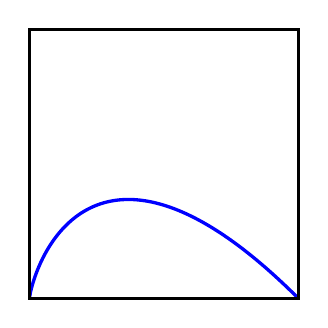
\begin{tikzpicture}
    \begin{axis}[
      % --- Box Style (maintaining consistency) ---
      axis line style={very thick},
      axis on top,
      enlargelimits=false,
      width=5cm,
      height=5cm,
      % Remove ticks and labels
      xtick=\empty,
      ytick=\empty,
      xlabel={},
      ylabel={},
      title={},
      % --- Axis Limits ---
      xmin=0, xmax=1,
      ymin=0, ymax=1, % A CDF always ranges from 0 to 1
      % --- Plot Style ---
      samples=200, % Sufficient for a smooth curve
      every axis plot/.append style={very thick, smooth}
      ]
      \addplot[blue, domain=0:1] {-x*ln(x)};
    \end{axis}
  \end{tikzpicture}
  \caption{The value of \(\phi(x)\) for \(0 \le x \le 1\).}
\end{figure}

\begin{definition}
  Let \(\mathcal{P}\) be a partition of \(X\). We say \(\mathcal{P}\) has \emph{finite entropy} if there is a countable subset \(\mathcal{P}' \subseteq \mathcal{P}\) for which \(\bigcup_{P \in \mathcal{P}'}P\) covers \(X\) modulo \(\mu\), and such that
  \begin{equation*}
    H_{\mu}(\mathcal{P}) = \sum_{P \in \mathcal{P}} \phi(\mu(P)) < \infty.
  \end{equation*}
  We call \(H_{\mu}(\mathcal{P})\) the \emph{entropy} of the partition \(\mathcal{P}\).
\end{definition}

\begin{definition}
  Let \((X,\mathcal{B},\mu,f)\) be a measure-preserving system and \(\xi\) be a partition of \(X\) with finite entropy. Then, the \emph{entropy of \(f\) with respect to \(\xi\)} is
  \begin{equation*}
    h_{\mu}(f,\xi) =
    \lim_{n \to \infty} \frac{1}{n}H_{\mu}\rpar*{\bigvee_{0 \le k < n}f^{-k}(\xi)} = 
    \inf_{n \ge 0} \frac{1}{n}H_{\mu}\rpar*{\bigvee_{0 \le k < n}f^{-k}(\xi)}.
  \end{equation*}
\end{definition}

\begin{definition}
  The \emph{entropy} of \(f\) with respect to \(\mu\) is defined as the supremum of the entropy of \(f\) with respect to partitions with finite entropy, that is,
  \begin{equation*}
    h_{\mu}(f) = \sup_{\xi \colon H_{\mu}(\xi) < \infty}h_{\mu}(f,\xi).
  \end{equation*}
\end{definition}

\subsection{Conditional entropy}

We also have a notion of \emph{conditional entropy}.

\begin{definition}
  Let \(\mathcal{P}\) be a partition of a Borel probability space \((X,\mathcal{B},\mu)\), and let \(\mathcal{A} \subseteq \mathcal{B}\) be a sub-\(\sigma\)-algebra. We define the \emph{conditional entropy} of \(\mathcal{P}\) given \(\mathcal{A}\) to be
  \begin{equation*}
    H_{\mu}(\mathcal{P}\mid \mathcal{A}) =
    \int H_{\mu^{\mathcal{A}}_x}(\mathcal{P}) \;d\mu(x),
  \end{equation*}
  where \(H_{\mu^{\mathcal{A}}_x}(\mathcal{P})\) is defined to be \(+\infty\) when \(\mathcal{P}\) is not of finite entropy for \(\mu^{\mathcal{A}}_x\).
\end{definition}

\begin{proposition}
  If \((X,\mathcal{B},\mu,f)\) if a measure-preserving system and \(\xi\) is a partition of \(X\) with finite entropy, the entropy of \(f\) with respect to \(\xi\) is equivalently equal to
  \begin{equation*}
    h_{\mu}(f,\xi) =
    \lim_{n \to \infty} \frac{1}{n}H_{\mu}\rpar*{\xi \mathrel{\bigg|} \bigvee_{1 \le k \le n}f^{-k}(\xi)}.
  \end{equation*}
\end{proposition}

\begin{proof}
  See~\cite[proposition 1.16]{einsiedlerEntropyErgodicTheory}.
\end{proof}

\subsection{Leddrapier-Young formula}

Let \(f \colon M \to M\) be a measure-preserving \(C^2\)-diffeomorphism of a compact \(C^{\infty}\) riemannian manifold \(x\) preserving an ergodic borel probability measure \(\mu\). By \cref{thm:oseledets} applied to \(\theta(x) = df_x\) and ergodicity of \(\mu\), we have a full-measure set \(\Gamma \subseteq M\), a positive integer \(r > 0\) and numbers \[\lambda_1 > \cdots > \lambda_r\] such that for all \(x \in \Gamma\), there is a filtration of the tangent bundle
\begin{equation*}
  \set{0} = V^0_x \subseteq V^1_x \subseteq \cdots \subseteq V^{r}_x = T_xM
\end{equation*}
where \cref{item:7,item:8} of \cref{thm:oseledets} apply. Let \(u = \max \set{i : \lambda_{i} > 0}\). For each \(1 \le i \le u\), define
\begin{equation*}
  W^i(x) = \set[par = \Big]{y \in M \where \limsup_{n \to \infty} \frac{1}{n} \log d(f^{-n}(x), f^{-n}(y))\le - \lambda_i }.
\end{equation*}
This is an immersed \(\dim V^i\)-dimensional \(C^2\) submanifold tangent at each point to \(V^i\)~\cite{ledrappierMetricEntropyDiffeomorphisms1985a}. It is called the \(i\)-th unstable manifold of \(f\) and \(x\), and it defines a foliation \(\set{W^i(x)}_{x \in X}\), called the \(i\)-th unstable foliation.

We now define a notion of dimension along the unstable foliation. Let \(1 \le i \le u\) and let \(\xi\) be a measurable partition of \(M\) that refines the foliation \(W^i\). For \(x \in M\), let \(\mu_x\) be the conditional measure at \(x\) for the partition \(\xi\), and let
\begin{equation*}
  \underline{\delta}_i(x,\xi) = \liminf_{\varepsilon \to 0}\frac{\log \mu_x (B^i(x,\varepsilon))}{\log \varepsilon}
\end{equation*}
and
\begin{equation*}
  \overline{\delta}_i(x,\xi) = \limsup_{\varepsilon \to 0}\frac{\log \mu_x (B^i(x,\varepsilon))}{\log \varepsilon}
\end{equation*}

\begin{lemma}
  The functions \(\underline{\delta}_i(x,\xi)\) and \(\overline{\delta}_i(x,\xi)\) are invariant by \(f\) and independent of \(\xi\), and therefore are almost everywhere equal to two numbers \(\underline{\delta}_i\) and \(\overline{\delta}_i\). In fact, these two numbers are equal, and we denote the common value by \(\delta_i\).
\end{lemma}

\begin{proof}
  See~\cite{ledrappierMetricEntropyDiffeomorphisms1985a}.
\end{proof}

The number \(\delta_i\) is called the \emph{dimension of \(\mu\) on \(W^i\)-manifolds}.

\begin{theorem}[Ledrappier-Young formula]\label{thm:leddrappier-young}
  Let \(\lambda_1 > \cdots > \lambda_u > 0\) be the distinct positive Lyapunov exponents of \(f\) for \(\mu\), and let \(\delta_i\) be the dimension of \(\mu\) on \(W^i\)-manifolds. Then, for all \(1 \le i \le u\) there exist real numbers \(0 \le \gamma_i \le \dim V^i - \dim V^{i - 1}\) such that
  \begin{equation*}
    \delta_i = \sum_{j \le i} \gamma_i
  \end{equation*}
  and
  \begin{equation*}
    h_{\mu}(f) = \sum_{i \le u} \lambda_i\gamma_i.
  \end{equation*}
\end{theorem}

\begin{proof}
  See~\cite{ledrappierMetricEntropyDiffeomorphisms1985a}.
\end{proof}

\end{document}
